\documentclass[
    a4paper,
    11pt
]{article}

\usepackage[utf8]{inputenc}
\usepackage{float}
\usepackage{mathtools}
\usepackage{amssymb}
\usepackage{physics}
\usepackage{tabulary}
\usepackage{booktabs}
\usepackage{graphicx}


\begin{document}

\tableofcontents

\clearpage

\section{General}

\subsection{Taylor Series}

One-dimensional Taylor-Series Expansion for a n+1 continously differentiable
function on the the interval a to b with a $\xi \in [x, x+h]$
\begin{equation}
    f(x+h) = \sum_k^n \frac{1}{k!} f^{(k)}(x)h^k + \frac{1}{(n+1)!}
    f^{(n+1)}(\xi)h^{n+1}
\end{equation}

\subsection{Implicit Function Theorem}

\subsection{Total Derivative}

\subsection{Gershgorin Disks}

Gershgorin disks give an estimate to where eigenvalues of a matrix lie in the
complex plain. Assume $A \in \mathbb{C}^{n x n}$
\begin{equation}
    R_i := \left\{z \in{} \mathbb{C} |
    |z - a_{ii}| \leq{} \sum_{\substack{j=1 \\ j\neq{} i}}^{n}|a_{ij}| \right\}
\end{equation}
The the set of z (=R) describe the Gershgorin disks in which the eigenvalue can
be found

%%% ---------------------

\section{Polynomials}

\subsection{Monomial Basis}

\begin{equation}
    span\{1, x, x^2, x^3, ..., x^n\} = \Pi_n
\end{equation}

\subsection{Lagrange Polynomials}

On a set of points $t_i$ these polynomials are zero at $k \neq j$ and 1 at $k =
i$
\begin{equation}
    L_k(t) := \prod_{\substack{i=0 \\ i\neq j}}^{n} \frac{t - t_i}{t_k - t_i}
    \in \Pi_n
\end{equation}

\subsection{Chebychev Polynomials}

The Chebychev polynomials are directly defined by
\begin{equation}
    T_n(x) = \cos(n\arccos(x))
\end{equation}

Or by a three term recursion (it shares the first two polynomials with the
common monomial basis)
\begin{equation}
    T_n(x) = 2xT_{n-1}(x) - T_{n-2}(x), \quad T_0(x) = 1, \quad T_1(x) = x
\end{equation}

\subsection{Hermite Polynomials}

Require position and slope at each point. Can be used for Hermite cubic spline
interpolation, however then only $C^1$ over the nodes

\subsection{Legendre Polynomials}

The Legendre Polynomials form a basis of the space of polynomials and are
directly defined by
\begin{equation}
    P_n(x) = \frac{1}{2^n n!} \dv[n]{}{x}[(x^2 - 1)^n]
\end{equation}

The recursive definition is given by
\begin{equation}
    (n+1)P_{n+1}(x) = (2n+1)xP_n(x) - n P_{n-1}(x), \quad P_0 = 1, \quad P_1=x
\end{equation}


%%% ----------------------------------

\section{Error Analysis}

General Relative condition nuumber for $\mathbf{f}:\mathbb{R}^n -> \mathbb{R}^m$ if the
peturbed input $\mathbf{\tilde{x}}$ approaches the non-perturbed
\begin{equation}
    \frac{||\mathbf{f}(\mathbf{x}) -
    \mathbf{f}(\mathbf{\tilde{x}})||}{||\mathbf{f}(\mathbf{x})||} \le
    \kappa_{rel}(\mathbf{f})(\mathbf{x}) \cdot
    \frac{||\mathbf{x} - \mathbf{\tilde{x}}||}{||\mathbf{x}||}
\end{equation}

Additionally, one has to outfit both multidimensional quantitities with a
corresponding norm (idealls, it is the same type of norm for both). If the
function is continously differentiable we get the first order approximation to
\begin{equation}
    \kappa_{rel}(\mathbf{f})(\mathbf{x}) \dot{=}
    \frac{||\mathbf{x}||}{||\mathbf{f}(\mathbf{x})||}
    ||\mathbf{f}'(\mathbf{x})||
\end{equation}

Where the derivative of the function is its Jacobian. Therefore, one has to
define an appropriate matrix norm.

\begin{figure}[H]
    \centering
    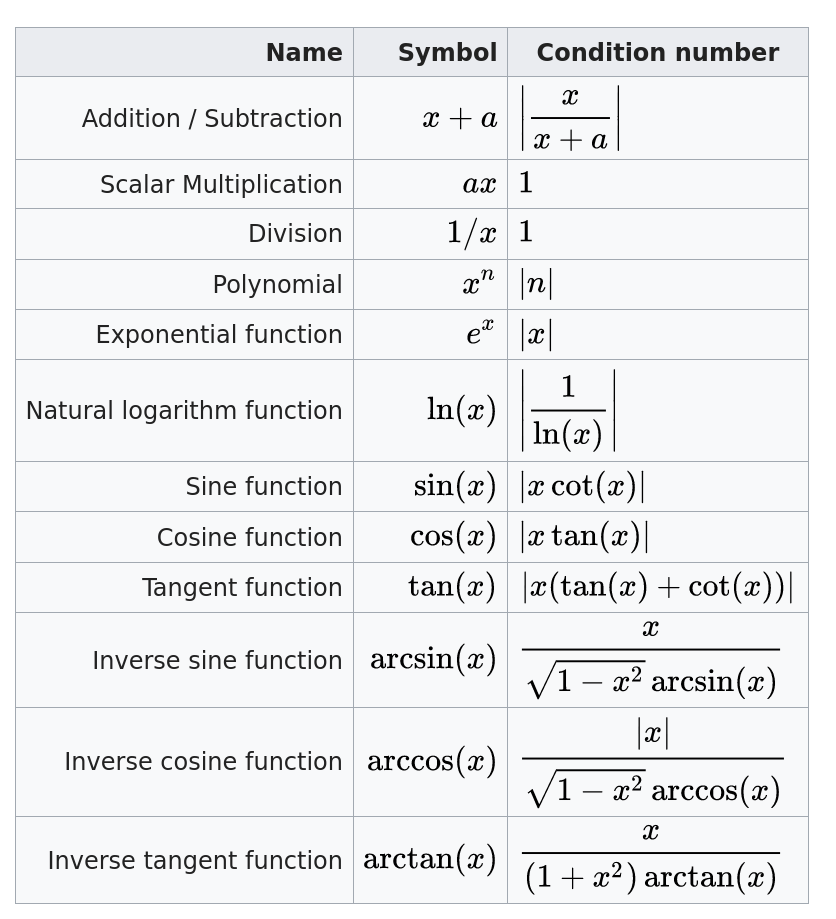
\includegraphics[width=0.5\linewidth]{basicOperations.png}
    \caption{Overview of relative condition number of basic operations.}
\end{figure}

Relative condition number of a multi-variant problem with one-dimensional output

\begin{equation}
    \kappa_{rel}(f, \vec{x}) =
    \frac{
        \sum_{i=1}^{n} \left| f_{x_i}(\vec{x}) \right| \cdot |x_i|
    } {
        \left| f(\vec{x}) \right|
    }
\end{equation}

Condition number of a matrix (e.g. choose the infinity matrix norm - row sum
norm)
\begin{equation}
    \kappa_{rel}(A) = ||A|| \cdot ||A^{-1}||
\end{equation}

\

\subsection{Loss of significant digits}

\begin{equation}
    \text{loss} = log_{10}(\kappa_{rel})
\end{equation}


\section{Matrix Factorization}

\subsection{QR Decompostion with Householder transformations}

Householder transformations are unitary and hermitian.

\begin{equation}
    \mathbf{T}^{-1} = \mathbf{T}^H = \mathbf{T} = I_n - 2
    \frac{\vec{u}\vec{u}^H}{\vec{u}^H\vec{u}} \in \mathbb{C}^{n x n}
\end{equation}

\subsection{Cost of Decompositions}

\begin{itemize}
    \item $\mathbf{LU} \propto 2\frac{n^3}{3}$
    \item Householder $\mathbf{QR} \propto 4\frac{n^3}{3}$
    \item Givens $\mathbf{QR} \propto 6\frac{n^3}{3}$

\end{itemize}

\section{Polynomial Interpolation}

\subsection{Direct - Barycentric Lagrange Interpolation}


Better stability properties than regular Lagrangian interpolation.

\subsection{Recursive - Aitken-Neville Algorithm}

Polynomial interpolation with Aitken-Neville of a set of $n+1$ data points to
interpolate a polynomial of degree $n$ in the form $P(x) = p_{0,n}(x)$. Start by
setting the initial values in the recursive scheme to $p_{i,i}(x)=y_i$. Then
calculate the other values by:
\begin{equation}
    p_{i,j}(x) = \frac{(x-x_j)p_{i,j-1}(x) - (x-x_i)p_{i+1,j}(x)}{x_i - x_j}
\end{equation}

More efficient evaluation of the Aitken-Polynomial at one certain point
\begin{equation}
    see matlab
\end{equation}

Aitken's theorem states that if two polynomial functions $M(t)$ and $N(t)$
interpolate $n-2$ common points, and $M(t)$ is additionally interpolating a
point before all the others and $N(t)$ is addtionally interpolating a point at
the end of the interval, then there is a unique polynomial $P(t)$ that
interpolates all value pairs as follows
\begin{equation}
    P(t) = N(t) + \frac{t - t_k}{t_k - t_i} (N(t) - M(t))
\end{equation}

\subsection{Recursive - Newton Algorithm}

Newton's Method provides a nice evalutation of a polynomial interpolation at
many points since it easily gives you the functional form of the interpolating
polynomial. Define the divided differences

\begin{equation}
    f[t_i, t_{i+1}, ..., t_k] =
    \frac{f[t_{i+1}, ..., t_k] - f[t_i, ..., t_{k-1}]}{t_k - t_i},
    \quad
    f[t_i] := f(t_i) = y_i
\end{equation}

Then the polynomial is defined as
\begin{equation}
    P(t) = \sum_{k=0}^{n} f[t_0, ..., t_k] \prod_{i=0}^{k-1}(t - t_i)
\end{equation}

\subsection{Horner's scheme for efficient evaluation}

Using Horner's scheme, the polynomial can be evaluated more efficiently
\begin{verbatim}
    P_n := f[t_0, t_1, ..., t_n]
    k=n-1:-1:0:
        P_k := P_{k+1} * (t - t_k) + f[t_0, t_1, ..., t_k]
\end{verbatim}



\subsection{Chebychev nodal support for converging interpolation}

Chebychev nodes on an interval from $(a,b)$. $n$ nodes with index $k$. They are
the roots of the Chebychev polynomial of degree n.
\begin{equation}
    x_k = \frac{1}{2}(a+b) + \frac{1}{2}(b-a)\cos(\frac{2k-1}{2n}\pi)
\end{equation}

\subsection{Cubic Splines}

For efficient evaluation of cubic splines, use a different basis instead of the
standard monomial one (where we would have to solve for all 4 coefficients on
each sub-interval) - This basis has no special name
\begin{equation}
    \Pi_3 = \text{span}\left\{
        1 - \xi,
        \xi,
        -\frac{\xi}{3}+\frac{\xi^2}{2}-\frac{\xi^3}{6},
        -\frac{\xi}{6} + \frac{\xi^3}{6}
    \right\}, \quad \xi = \frac{t-t_i}{t_{i+1} - t_i}
\end{equation}

Then the interpolating polynomial is given by

\begin{equation}
    s_3(t) = y_i(1-\xi) + y_{i+1}\xi + h_i^2 y_i^{''} \left( -\frac{\xi}{3} +
    \frac{\xi^2}{2} - \frac{\xi^3}{6} \right) + h_i^2 y_{i+1}^{''} \left(
    -\frac{\xi}{6} + \frac{\xi^3}{6} \right)
\end{equation}

This is beneficial since $y_i$ is already available due to the inerpolating
condition. The second derivatives at each node can be efficiently computed.
Introduce the following abbreviations ($\mu_i + \lambda_i =1$)

\begin{equation}
    \mu_i := \frac{h_{i-1}}{h_{i-1} + h_i} = \frac{t_i -t_{i-i}}{t_{i+1} -
    t_{i-1}} > 0
\end{equation}
\begin{equation}
    \lambda_i := \frac{h_i}{h_{i-1} + h_i} = \frac{t_{i+1} - t_i}{t_{i+1} -
    t_{i-1}} > 0
\end{equation}

Then the following triagonal (non-square since we have 2 DoF) system has to be
solved

\begin{equation}
    \mu_i y_{i-1}^{''} + 2y_i^{''} + \lambda_i y_{i+1}^{''} = 6 y_{i-1,i,i+1}
\end{equation}

This creates $(n-2) x n$ system for the $n-2$ interior nodes. It uses the second
devided difference (refer to Newton's interpolation scheme) defined by

\begin{equation}
    y_{i-1,i,i+1} = \frac{y_{i,i+1} - y_{i-1,i}}{h_{i-1} + h_i}
\end{equation}

With the regular divided differenc given by

\begin{equation}
    y_{i, i+1} = \frac{y_{i+1} - y_i}{h_{i}}
\end{equation}

This system is underconstrained. We have to prescribe boundary conditions. These
can be of following type

\begin{itemize}
    \item Hermite splines $s_3^{'}(t_0) = y_0^{'}$ and $s_3^{'}(t_n) = y_n^{'}$ are
        prescribed
    \item $s_3^{''}(t_0) = y_0^{''}$ and $s_3^{''}(t_n) = y_n^{''}$ are
        prescribed. "Natural Spline" if both are set to zero.
    \item Periodic Splines $s_3^{'}(t_0) = s_3^{'}(t_n)$ and $s_3^{''}(t_0) =
        s_3^{''}(t_n)$ are prescribed
\end{itemize}

By the help of the Gershgorin Disks we can proof that under a given bounary
condition the cubic spline is unique.

The erros for the different derivatives are given

...

By this we can conclude that that the splines converge against the function they
are interpolating for increasingly finer subintervals. For Polynomials this is
not given (only on Chebychev nodes).

\subsection{Cost of interpolation}

\begin{itemize}
    \item Barycentric Lagrange: Computing weights $\propto n^2$, adding value
        $\propto n$, evaluating polynomial $\propto n$
    
\end{itemize}


%%% ------
\section{Trigonometric Interpolation}

\subsection{Discrete Fourier Transform (DFT)}

\subsection{Fast Fourier Transform (FFT)}


%%% --------------------
\section{Quadrature - Numerical Integration}

\subsection{Newton-Cotes-Methods}

Newton-Cotes type quadrature interpolates the integrand by the help of
polynomials on an equidistant grid. Composite rules define their sub-interval
length to $\frac{b-a}{n}$ with n sub-intervals.


\begin{table}[H]
    \centering
    \begin{tabulary}{\linewidth}{C C C}
        \toprule
        name & definition & remainder\\
        \midrule
        Trapezoid &
            $\displaystyle \frac{b-a}{2} (f(a) + f(b)) $ &
            $\displaystyle -\frac{f^{''}(\eta)}{12}(b-a)^3$
        \\
        Kepler &
            $\displaystyle \frac{b-a}{6} \left( f(a) + 4f(\frac{a+b}{2}) + f(b)
            \right)$ &
            $\displaystyle - \frac{f^{(4)}(\eta)}{90} \left(\frac{b-a}{2}
            \right)^5$
        \\
        \midrule
        Comp. Trapez. &
            $\displaystyle \frac{h}{2} \left( f(a) + 2 \sum_{j=1}^{n-1}f(x_j) +
            f(b) \right) $ &
            $\displaystyle - \frac{b-a}{12} h^2 f^{''}(\eta)$
        \\
        Simpson &
            $\displaystyle \frac{h}{3} \sum_{j=1}^{n/2} \left[ f(x_{2j-2}) + 4
            f(x_{2j-1}) + f(x_{2j}) \right] $ &
            $\displaystyle - \frac{h^4}{180}(b-a) f^{(4)}(\eta)$
        \\

        \bottomrule

    \end{tabulary}
\end{table}

\subsection{Adaptive Composite Rules}

\begin{itemize}
    \item Start with course sub-intervals $h_1$
    \item Half the sub-interval-lengths everywhere $h_2=h_1/2$
    \item For each interval calculate the error $err_j = |S_{\text{coarse}} -
        S_{\text{fine}}|$
    \item Weight each error with the sub-interval length $err_j \frac{h_j}{b-a}$
    \item Refine the sub-intervals further (recursively) if error is above a set
        tolerance
\end{itemize}



%%% --------------
\section{Eigenvalues}

Eigenvalues should numerically never be determined by the roots of the
characteristic polynomial. Instead use other algorithms like (inverse) power
iteration or the QR algorithm. Then the condition number of finding an
eigenvalue is given as

\begin{equation}
    \kappa(\lambda) = ||\mathbf{V}||\cdot||\mathbf{V}^{-1}||
\end{equation}
With the eigenvector matrix $\mathbf{V}$. If the matrix $\mathbf{A}$ is normal,
i.e. $\mathbf{AA}^H = \mathbf{A}^H \mathbf{A}$, then $\mathbf{V}$ is unitary and
the problem is perfectly conditioned.
\end{document}
